
\documentclass[a4paper,12pt]{article} % добавить leqno в [] для нумерации слева

\usepackage[left=2cm,right=2cm,
top=2cm,bottom=2cm,bindingoffset=0cm]{geometry}


\usepackage{cmap}

\usepackage{amsmath,amsfonts,amssymb,amsthm,mathtools} % AMS
\usepackage{mathtext}
\usepackage[TS1,T2A]{fontenc}
\usepackage[utf8]{inputenc}
\usepackage{siunitx}

\usepackage[english,russian]{babel}

\usepackage{fontspec}         % пакет для подгрузки шрифтов

\setmainfont{Times New Roman}       % задаёт основной шрифт документа


\usepackage{icomma} 
\mathtoolsset{showonlyrefs=true} % Показывать номера только у тех формул, на которые есть \eqref{} в тексте.
\usepackage{euscript}	 % Шрифт Евклид
\usepackage{mathrsfs} % Красивый матшрифт
\usepackage{enumitem}
\usepackage{tikz} % To generate the plot from csv
\usepackage{pgfplots}

\usepackage{multicol}
\setlength{\columnsep}{1cm}

%\renewcommand{\theenumi}{(\Asbuk{enumi})}
%\renewcommand{\labelenumi}{\Asbuk{enumi})}

\makeatletter
\AddEnumerateCounter{\asbuk}{\russian@alph}{щ}
\makeatother

%%% Заголовок
\author{Касьянова Ксения, Федорчук Яна (ЭО-15-01) }
\title{Домашнее задание 1}
\date{\today}


\begin{document}

\maketitle

\subsubsection*{(а)}	
	
Оценим регрессию логарифма ВВП по индексу институтов с помощью МНК.
	
	
\begin{table}[h!]
	\centering
	\begin{tabular}{rrrrr}
		\hline
		& Estimate & Std. Error & t value & Pr(>|t|) \\ 
		\hline
		(Intercept) & 4.6604 & 0.4085 & 11.41 & 0.0000 \\ 
		prot & 0.5221 & 0.0612 & 8.53 & 0.0000 \\ 
		\hline
	\end{tabular}
\end{table}	
	
\begin{figure}[h!]
	\centering
	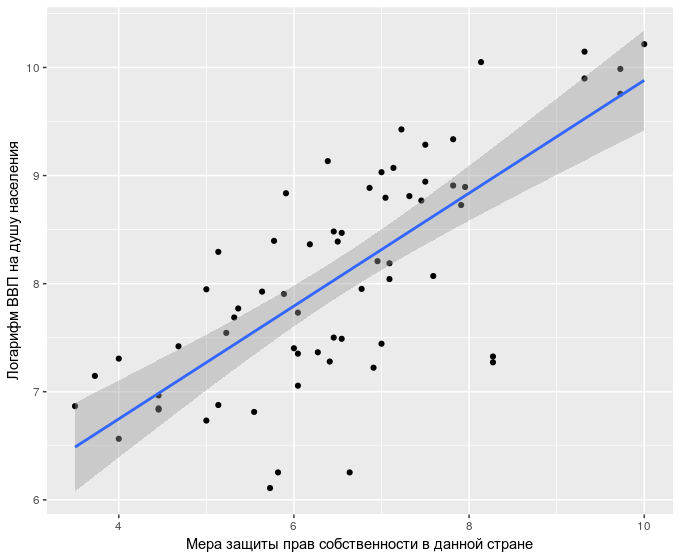
\includegraphics[width=0.7\linewidth]{Rplot1}
	\caption[Диаграмма рассеяния]{Диаграмма рассеяния}
	\label{fig:rplot1}
\end{figure}



Полученная зависимость не может быть интерпретирована как
причинно-следственная связь из-за  эндогенности  регрессора. 
Причины несостоятельности оценки коэффициента при переменной prot:
\begin{enumerate}
	\item Двусторонняя причинно-следственная связь
\item Пропущенные переменные
\item Ошибки измерения регрессора
\end{enumerate}	
	
	
\subsubsection*{(б)}	

Оценим регрессию логарифма ВВП по индексу институтов и широте  с помощью МНК.


\begin{table}[h!]
	\centering
	\begin{tabular}{rrrrr}
		\hline
		& Estimate & Std. Error & t value & Pr(>|t|) \\ 
		\hline
		(Intercept) & 4.7281 & 0.3973 & 11.90 & 0.0000 \\ 
		prot & 0.4679 & 0.0642 & 7.29 & 0.0000 \\ 
		latitude & 1.5769 & 0.7103 & 2.22 & 0.0301 \\ 
		\hline
	\end{tabular}
\end{table}


При добавлении latitude в качестве регрессора  
оценка коэффициента при индексе институтов prot практически не изменяется. Сама переменная статистически значима и имеет положительный знак.



\subsubsection*{(в)}	

Оценим регрессию логарифма ВВП по смертности поселенцев  с помощью МНК.

\begin{table}[h!]
	\centering
	\begin{tabular}{rrrrr}
		\hline
		& Estimate & Std. Error & t value & Pr(>|t|) \\ 
		\hline
		(Intercept) & 10.7076 & 0.3748 & 28.57 & 0.0000 \\ 
		logmort & -0.5698 & 0.0780 & -7.30 & 0.0000 \\ 
		\hline
	\end{tabular}
\end{table}

\begin{figure}[h!]
	\centering
	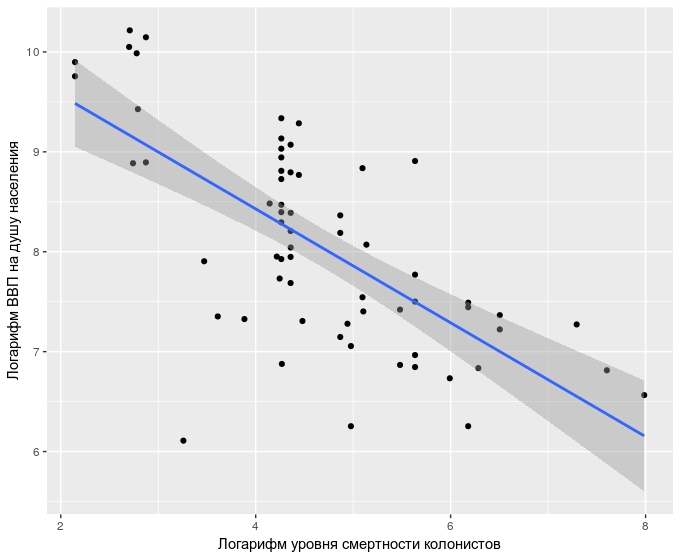
\includegraphics[width=0.7\linewidth]{Rplot2}
	\caption[Диаграмма рассеяния]{Диаграмма рассеяния}
	\label{fig:rplot1}
\end{figure}

Оценка коэффициента при переменной смертности меньше нуля, что верно согласно аргументам, приведенным в статье,  и логике: чем выше смертность колонистов, тем ниже будет ВВП в колониях, т.е. поскольку колонии, где европейцы сталкиваются с более высокими показателями смертности, сегодня значительно беднее колоний, которые были здоровы для европейцев. 

\newpage

\subsubsection*{(г)}	

Оценим регрессию логарифма ВВП по индексу институтов с помощью 2МНК, где инструментом является смертность  поселенцев.

\begin{table}[h!]
	\centering
	\begin{tabular}{rrrrr}
		\hline
		& Estimate & Std. Error & t-value & Pr(>|t|) \\ 
		\hline
		(Intercept) &  2.0869 &    0.9853 &  2.118 &  0.0382 \\ 
		prot & 0.9171  &   0.1502 &  6.106 & 0.0000 
		\\ 
		\hline
	\end{tabular}
\end{table}	

 Данный
инструмент можно  считать валидным, что 
позволяет корректно тестировать наличие причинно-следственной
связи между качеством институтов и ВВП, поскольку коэффициенты смертности европейских поселенцев более 100 лет назад не влияют на ВВП на душу населения сегодня, кроме их влияния за счет институционального развития. 
Также мы можем подтвердить, что наши результаты не обусловлены пропущенными факторами, т.е. нет других факторов, связанных с оценкой смертности поселенцев, влияющих на доход на душу населения: 
включение ряда переменных, которые потенциально коррелируют с летальностью поселенцев и экономическими результатами, не  отменяет наши результаты.
Невозможно контролировать все возможные переменные, которые могут быть коррелированы с летальностью поселенцев и экономическими результатами, а выбор нашего инструмента мог бы отразить влияние смертности поселенцев на экономические показатели через  другие каналы. Эти проблемы выявляются   с помощью  теста  Саргана.
 

\subsubsection*{(д)}	

Для первого шага 2МНК  оценим регрессию индекса институтов по смертности поселенцев  с помощью МНК.


\begin{figure}[h!]
	\centering
	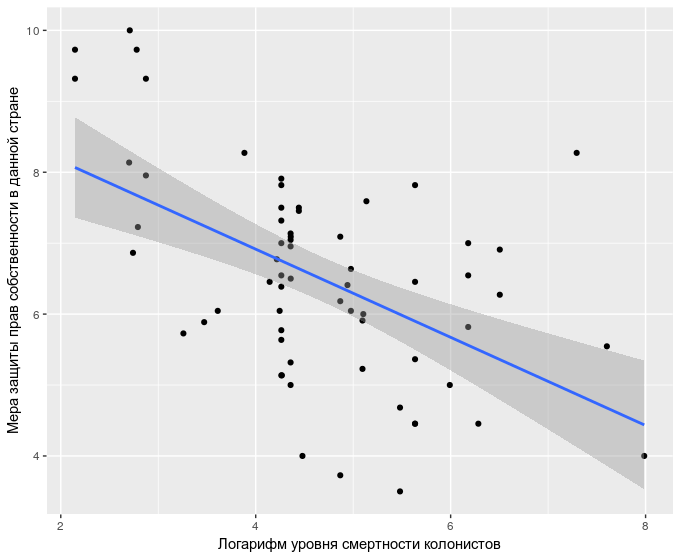
\includegraphics[width=0.7\linewidth]{Rplot3}
	\caption[Диаграмма рассеяния]{Диаграмма рассеяния}
	\label{fig:rplot1}
\end{figure}


\begin{table}[h!]
	\centering
	\begin{tabular}{rrrrr}
		\hline
		& Estimate & Std. Error & t value & Pr(>|t|) \\ 
		\hline
		(Intercept) & 9.4002 & 0.6116 & 15.37 & 0.0000 \\ 
		logmort & -0.6213 & 0.1273 & -4.88 & 0.0000 \\ 
		\hline
	\end{tabular}
\end{table}

Соответствующая F-статистика $ F = 23.82 $. Используемый инструмент является  релевантным, так как $ F > 10 $.


\subsubsection*{(е)}	

Для второго шага 2МНК  оценим регрессию 
логарифма ВВП по оценке  индекса институтов из первого шага с помощью МНК.

\begin{table}[h!]
	\centering
	\begin{tabular}{rrrrr}
		\hline
		& Estimate & Std. Error & t value & Pr(>|t|) \\ 
		\hline
		(Intercept) & 2.0869 & 0.8238 & 2.53 & 0.0138 \\ 
		prot\_est & 0.9171 & 0.1256 & 7.30 & 0.0000 \\ 
		\hline
	\end{tabular}
\end{table}

Оценка влияния качества институтов на ВВП по
сравнению с оценкой выросла c $ \beta_{OLS} = 0.5221 $ до  $ \beta_{2SLS} = 0.9171 $. Такое
изменение говорит о наличии пропущенных переменных как причины эндогенности в первоначальной модели.


\subsubsection*{(ё)}	

Оценим альтернативную регрессию логарифма ВВП по индексу институтов с помощью 2МНК, где инструментом является смертность  поселенцев, а контрольной переменной - широта.

\begin{table}[h!]
	\centering
	\begin{tabular}{rrrrr}
		\hline
		& Estimate & Std. Error & t-value & Pr(>|t|) \\ 
		\hline
		(Intercept) &   1.9358   &  1.2115  & 1.598  &  0.115  \\ 
		prot & 0.9533   &  0.2076 &  4.593 & 0.000 \\ 
		latitude &    -0.4685    & 1.2654 & -0.370  &  0.713
			\\ 
		\hline
	\end{tabular}
\end{table}	

Вывод, наблюдается устойчивое  положительое  влияние качества институтов на ВВП.


\subsubsection*{(ж)}

Проведем анализ отдельных подвыборок:   используем  данные по всем странам, кроме
африканских.

Оценим регрессию логарифма ВВП по индексу институтов с помощью 2МНК, где инструментом является смертность  поселенцев.

\begin{table}[h!]
	\centering
	\begin{tabular}{rrrrr}
		\hline
		& Estimate & Std. Error & t-value & Pr(>|t|) \\ 
		\hline
		(Intercept) & 4.56196  &  0.69211 &  6.591 & 0.0000  \\ 
		prot & 0.57685 &   0.09813  & 5.878 & 0.0000 
		\\ 
		\hline
	\end{tabular}
\end{table}	



Оценим альтернативную регрессию логарифма ВВП по индексу институтов с помощью 2МНК, где инструментом является смертность  поселенцев, а контрольной переменной - широта.


\begin{table}[h!]
	\centering
	\begin{tabular}{rrrrr}
		\hline
		& Estimate & Std. Error & t-value & Pr(>|t|) \\ 
		\hline
		(Intercept) &  0.57685  &  0.09813 &  5.878 & 0.000    \\ 
		prot & 0.57417  &  0.11726 &  4.896 & 0.000 \\ 
		latitude &   0.04407  &  0.83462 &  0.053  &  0.958   
		\\ 
		\hline
	\end{tabular}
\end{table}	




Теперь используем подвыборку только африканских стран. 

Оценим регрессию логарифма ВВП по индексу институтов с помощью 2МНК, где инструментом является смертность  поселенцев.

\begin{table}[h!]
	\centering
	\begin{tabular}{rrrrr}
		\hline
		& Estimate & Std. Error & t-value & Pr(>|t|) \\ 
		\hline
		(Intercept) & -3.576  &  14.716 & -0.243  &  0.810  \\ 
		prot & 1.858   &   2.504 &  0.742  &  0.465 
		\\ 
		\hline
	\end{tabular}
\end{table}	



Оценим альтернативную регрессию логарифма ВВП по индексу институтов с помощью 2МНК, где инструментом является смертность  поселенцев, а контрольной переменной - широта.


\begin{table}[h!]
	\centering
	\begin{tabular}{rrrrr}
		\hline
		& Estimate & Std. Error & t-value & Pr(>|t|) \\ 
		\hline
		(Intercept) &  -7.705 &    49.512 & -0.156  &  0.878  \\ 
		prot &  2.632   &   8.933 &  0.295 &   0.771 \\ 
		latitude &  -2.915  &   21.522 & -0.135 &   0.893   
		\\ 
		\hline
	\end{tabular}
\end{table}	




Сравним эффект воздействия качества институтов на ВВП на этой
подвыборке с оценками на базовой выборке. 
Мы подтверждаем, что оценки влияния институтов на эффективность не обусловлены выбросами, т.е. наши результаты  не изменяются при  исключении Африки. 

Данный эффект является гетерогенным, поскольку качество модели резко снижается при использовании подвыборки только с африканскими странами с $ multiple \ R^2_{without \ Africa} = 0.588   $ до $ multiple \ R^2_{with \ Africa} = -6.24  $  для первой модели и с $ multiple \ R^2_{without \ Africa} = 0.5894   $  до $ multiple \ R^2_{with \ Africa} = -14.11   $  для второй.   
	
\subsubsection*{(з)}	

Критик утверждает, что высокий ВВП на душу
населения 
объясняется прежде всего не качеством институтов, а высокой долей
населения европейского происхождения в общем населении этих стран.
Если критик прав и коэффициент при переменной euro будет значимой, то оценки в 2МНК уже не будут  состоятельными.
  


\subsubsection*{(и)}	

Проверим гипотезу, сформулированную критиком. 



Оценим регрессию логарифма ВВП по индексу институтов с помощью 2МНК, где инструментом является смертность  поселенцев, а контрольной переменной доля населения европейского происхождения в данной
стране.

\begin{table}[h!]
	\centering
	\begin{tabular}{rrrrr}
		\hline
		& Estimate & Std. Error & t-value & Pr(>|t|) \\ 
		\hline
		(Intercept) & 2.1550837 &  1.5465947 &  1.393& 0.168544    \\ 
		prot &  0.9049351 & 0.2539609 &  3.563& 0.000718 \\ 
		euro  &      0.0006053 & 0.0074203 &  0.082 &0.935256  
		 
		\\ 
		\hline
	\end{tabular}
\end{table}	



Оценим альтернативную регрессию логарифма ВВП по индексу институтов с помощью 2МНК, где инструментом является смертность  поселенцев, а контрольными переменной - широта доля населения европейского происхождения в данной
стране.

\newpage

\begin{table}[h!]
	\centering
	\begin{tabular}{rrrrr}
		\hline
		& Estimate & Std. Error & t-value & Pr(>|t|) \\ 
		\hline
		(Intercept) &  2.074465  &  1.623666 &  1.278 & 0.20630  \\ 
		prot &  0.931047 &  0.273167 &  3.408 & 0.00117 \\ 
		euro      &   0.001584 &  0.007742  & 0.205 & 0.83858   \\ 
		latitude &  -0.591921  &  1.195213 & -0.495 &  0.62224       
		\\ 
		\hline
	\end{tabular}
\end{table}	


В этих регрессиях ни расстояние от экватора, ни доля европейского населения не являются значимыми. Критик неправ. Эти результаты показывают, что некоторые страны  беднее других не из-за чистых географических или демографических  факторов, а из-за худших институтов.


	

\end{document}